\begin{figure*}[tb]
	\centering
	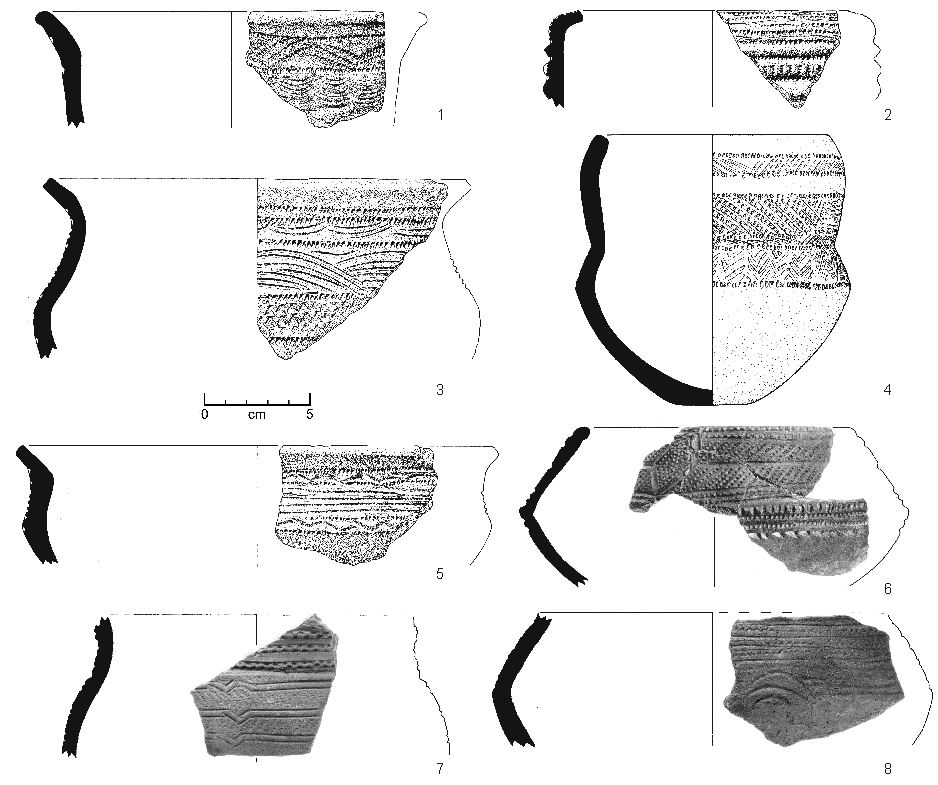
\includegraphics[width=\textwidth]{fig/MKL-Typen.pdf}
	\caption{Mokelo-Gruppe: Typvertreter aus Batanga (Fpl.~209), Mondoli (Fpl.~212), Mokelo (Fpl.~213) und Mboko~I (Fpl.~217).\\1:~Taf.~18.8; 2:~Taf.~18.1; 3:~Taf.~18.4; 4:~Taf.~18.3; 5:~Taf.~18.7; 6:~Taf.~17.4; 7:~Taf.~21.5; 8:~Taf.~16.3.}
	\label{fig:MKL_Typverteter}
\end{figure*}

\subsubsection{Mokelo-Gruppe}\label{sec:MKL-Gr}

Im Bereich des oberen \mbox{Ubangi} -- vornehmlich stromab des \mbox{Ubangi}-Bogens -- wurde bei Ober"-fl"-äch"-en-Surveys eine ritz- und rouletteverzierte Keramik entdeckt, die sowohl formale Ähnlichkeiten zur Batalimo-Maluba- (Kap.~\ref{sec:BTM-Gr}) und \mbox{Ngbanja}-Gruppe (Kap.~\ref{sec:NGB-Gr}) als auch zur Mot"-en"-go-Boma-Gruppe (Kap.~\ref{sec:MTB-Gr}) aufweist. Die Quellenlage für die formale Beschreibung dieser als Mokelo-Stil benannten Gruppe umfasst lediglich 49~GE sowie 36 ausgezählten Stücken aus zusammengenommen zehn verschiedenen Fundstellen. Das Gros der Funde stammt dabei vom eponymen Fundort Mokelo (Fpl.~213) sowie aus dem Dorf Mboko~I (Fpl.~217). 18~GE konnten nur unter Vorbehalt der Stilgruppe zugewiesen werden und bei einer weiteren GE war eine Unterscheidung zur Stilgruppe Motenge-Boma nicht zweifelsfrei möglich. Das Material wurde bislang in keiner Grabung erfasst, alle Funde stammen aus Absammlungen von Dorfflächen. Die Keramik der Mokelo-Gruppe fällt neben häufigen Ritz- und Eindruckmustern, die in einigen Fällen von Schnitzroulette begleitet werden, durch deutlich abknickende Gefäßwandungen auf (Abb.~\ref{fig:MKL_Typverteter}).

\paragraph{Technologische Merkmale}\hspace{-.5em}|\hspace{.5em}%
Die Mokelo-Keramik weist sehr heterogene Scherben auf. Die am häufigsten vertretenen \textit{Fabrics} sind 4a (16\,\%), 7d (12\,\%), 7c (12\,\%) sowie 5c (12\,\%). Der Anteil nichtplastischer Partikel in den Scherben liegt regelhaft zwischen 7--10\,\% und 25--40\,\%. Größtenteils handelt es sich um heterogene Mischungen von Quarzsanden, in einigen Fällen wurde aber auch Glimmer, Schamott, Laterit oder Organik in den Scherben beobachtet. Die zur Herstellung der Mokelo-Keramik genutzten Tone weisen häufig eine rote Brennfarbe auf. Eine größere Anzahl der Stücke konnte aufgrund schwarzer, grauer oder beiger Färbungen nicht dediziert angesprochen werden. Stücke, die auf die Nutzung weißbrennender Tone hinweisen, ließen sich nur selten beobachten. Alle GE wiesen eine gut geglättete Oberfläche auf.


\paragraph{Formen}\hspace{-.5em}|\hspace{.5em}%
Bei insgesamt 33~GE, die der Mokelo-Gruppe zugewiesen werden konnten, wurde auch die Gefäßform angesprochen. Das Formenspektrum ist deutlich heterogen. Den größten Anteil machen leicht bauchige Gefäße (Typ~C1; 18\,\%; Abb.~\ref{fig:MKL_Typverteter}.7), Schalen mit einbiegendem Rand (Typ~H2; 12\,\%; Taf.~18.10--11) sowie flache, leicht bauchige Gefäße mit kurzem Hals (Typ~E4; 12\,\%; Abb.~\ref{fig:MKL_Typverteter}.3, 5) aus. Ein eindeutiger Fokus auf spezifische Gefäßformen konnte nicht beobachtete werden. Unter Berücksichtigung der Grundformen sind leicht bauchige Töpfe (Typ~C), flache Töpfe (Typ~E), Töpfe mit Bauchknick (Typ~F), Schalen mit Bauchknick (Typ~G) sowie Schalen mit einbiegenden Rändern (Typ~H) in etwa gleichen Anteilen vertreten.

Die Bauchbereiche der Gefäße sind häufig mit einem deutlichen, scharfen Bauchknick  umgebrochen (33\,\%; Abb.~\ref{fig:MKL_Typverteter}.3, 4, 6, 8). Daneben kommen runde (27\,\%; Abb.~\ref{fig:MKL_Typverteter}.7) und flache Bauchbereiche (12\,\%) vor. Gerade die deutlich abknickenden Gefäßbäuche stachen bei der Durchsicht des Materials als diagnostisches Charakteristikum hervor. Während sich die runden Gefäßbäuche vornehmlich bei offenen Gefäßformen mit einbiegendem Rand zeigen, sind scharfe Bauchknicke bei verschiedenen Grundformen zu beobachten. Aus dem bestimmten Material heraus lassen sich aufgrund der geringen Anzahl von Beobachtungen -- in der Regel nur ein oder zwei Stücke je Klasse -- sowie der ausnahmslosen Herkunft des Materials aus Oberflächenabsammlungen keine klaren Muster ableiten.

Über die Hälfte der Ränder der Mokelo-Gruppe weisen einen rund ausgeführten Randabschluss auf (48\,\%), während gerillte (14\,\%) oder spitze Mündungen (10\,\%) deutlich seltener vertreten sind. Die Ränder, insgesamt konnte lediglich bei 31~GE der Mokelo-Gruppe eine Randform bestimmt werden, sind sehr heterogen. Die größte Gruppe mit 29\,\% (9~GE) sind einfach ausbiegende Ränder vom Typ B1 (Abb.~\ref{fig:MKL_Typverteter}.1, 3, 5). An den übrigen 22~GE konnten zwölf verschiedene Randformen beobachtet werden, die jeweils nur zwischen vier bis einmal auftraten. Eine klare Charakterisierung anhand der Randformen ist für die Mokelo-Gruppe nicht möglich. Eine GE, die einzige bei der die Bodenform angesprochen werden konnte, zeigt einen flachen Boden vom Typ B4 (Abb.~\ref{fig:MKL_Typverteter}.4).

\begin{figure*}[p]
\centering
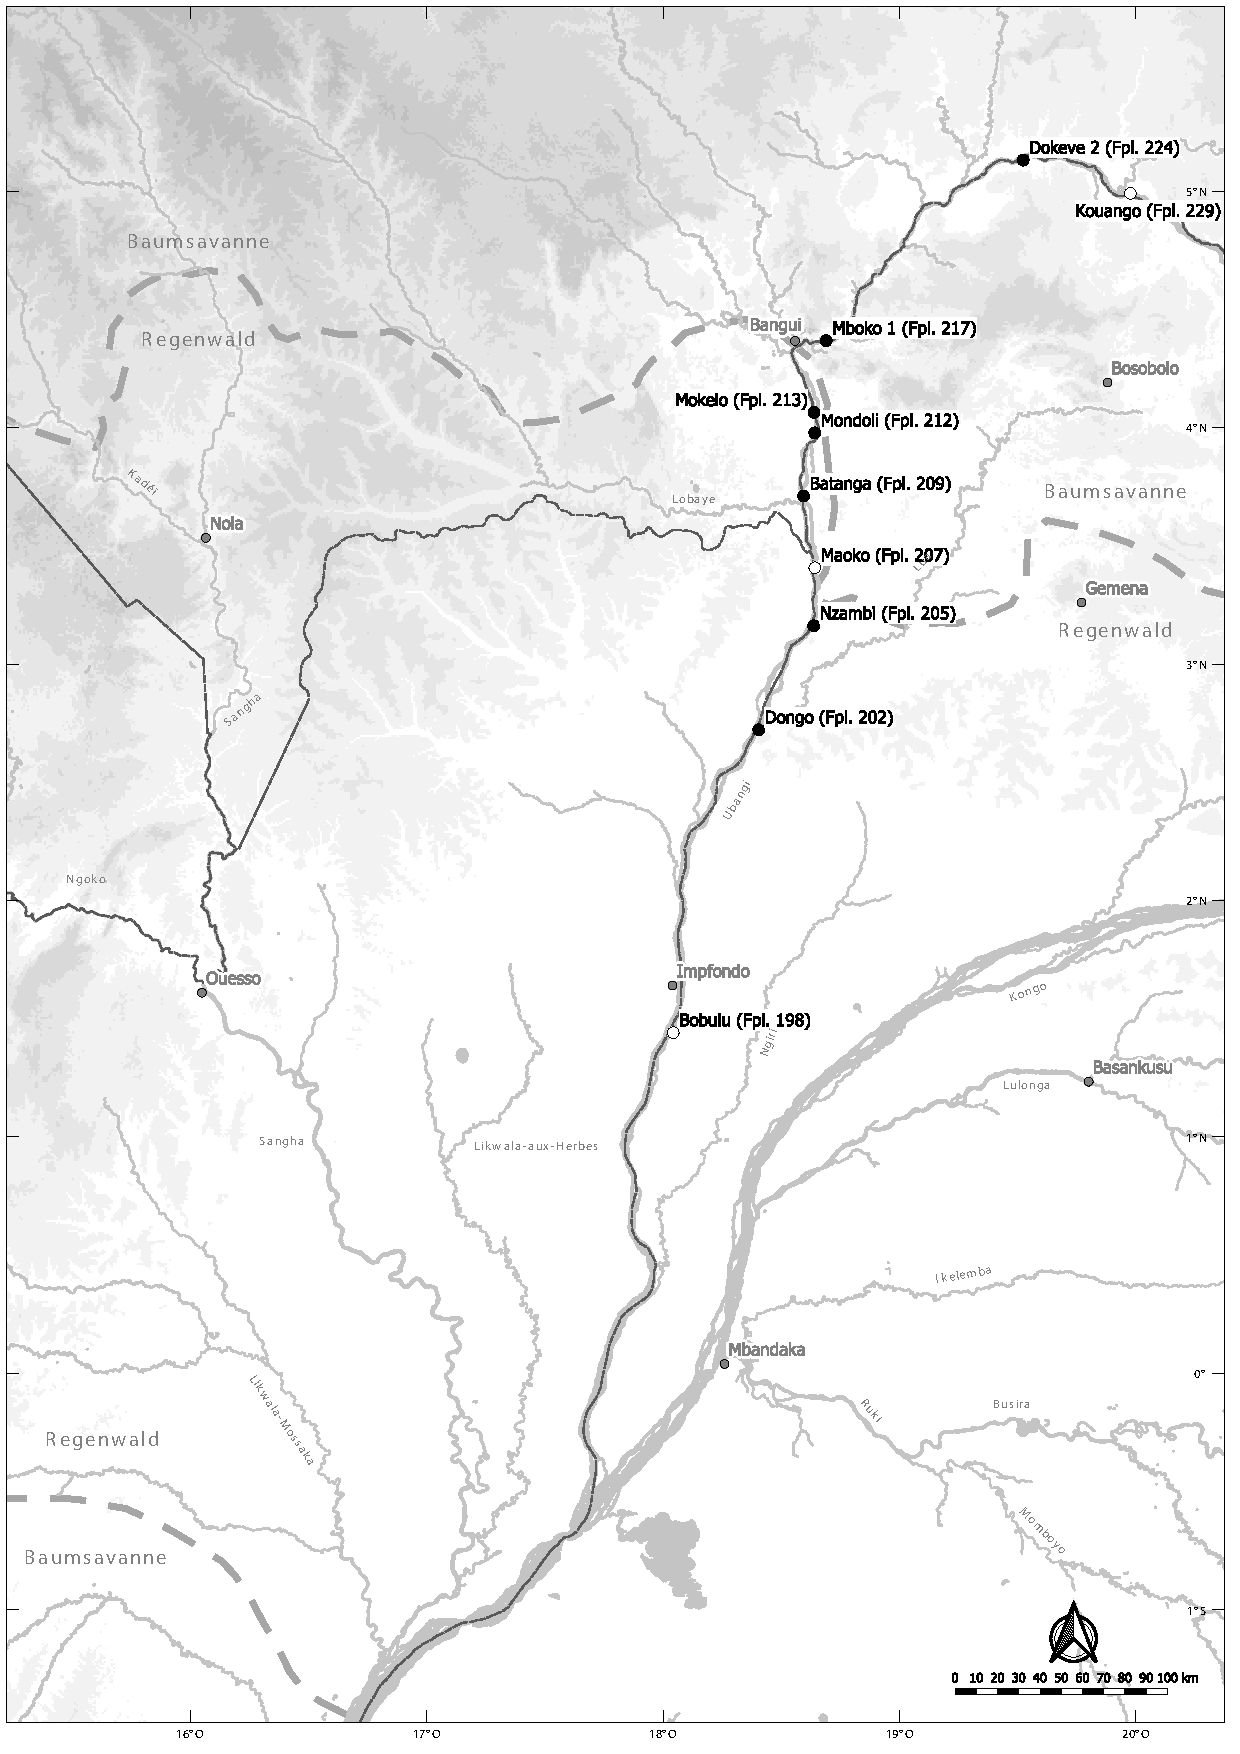
\includegraphics[width=\textwidth]{fig/MKL_Verbreitung.pdf}
\caption{Mokelo-Gruppe: Verbreitung.}
\label{fig:MKL_Verbreitung}
\end{figure*}

\paragraph{Verzierungen}\hspace{-.5em}|\hspace{.5em}%
Die Keramik der Mokelo-Gruppe wird vor allem durch drei Verzierungselemente charakterisiert (Anlage~4\subref{fig:MKL_Verz}): horizontale Rillen (Tab.~\ref{tab:Verzierungselemente}: 02.1; 23\,\%), diagonale Bänder (Tab.~\ref{tab:Verzierungselemente}: 05.1; 10\,\%) und horizontale Reihen aus Eindrücken eines Kamms oder einzinkigen Gerätes (Tab.~\ref{tab:Verzierungselemente}: 04.11; 35\,\%). In deutlich geringerem Maße kommen weitere Verzierungselemente, unter anderem vegetabilische oder Schnitzroulette, vor. Die verschiedenen Rouletteverzierungen machen zusammen lediglich 4\,\% aller beobachteten Verzierungselemente aus. Vegetabilisches \mbox{Roulette} wurde an lediglich zwei GE beobachtet, während fünf GE Schnitzroulette aufwiesen. Ebenfalls seltene Verzierungselemente sind Zickzack-Muster (Tab.~\ref{tab:Verzierungselemente}: 01.6; 5\,\%) beziehungsweise Bänder aus Zickzack-Kammeindrücken (Tab.~\ref{tab:Verzierungselemente}: 05.02; 3\,\%) sowie bogenförmige Riefen (Tab.~\ref{tab:Verzierungselemente}: 02.5; 5\,\%).

Die Verzierungen finden sich grundsätzlich auf den oberen Bereichen der Gefäße, eine Verzierung der Standflächen konnte in keinem Fall und die eines Bodenansatzes nur bei einer GE beobachtet werden (Anlage~4\subref{fig:MKL_Verz}). Die Innenseiten sind ebenfalls nur äußerst selten verziert. Keine der drei weiter oben genannten, bestimmenden Verzierungselemente (Tab.~\ref{tab:Verzierungselemente}: 02.1, 05.1 und 04.11) zeigt eine Begrenzung auf eine bestimmte Gefäßposition, sie finden sich regelhaft auf den oberen Gefäßbereichen.


\paragraph{Datierung}\hspace{-.5em}|\hspace{.5em}%
Für das unter der Bezeichnung Mokelo zusammengefasste Fundmaterial liegen keine absoluten Daten vor. Die Keramik der Mokelo-Gruppe weist eine Reihe von Merkmalen auf, die sie mit weiteren keramischen Stilgruppen entlang des \mbox{Ubangi} in Verbindung setzt. Die deutliche S-Profilierung vieler Gefäße sowie die Nutzung von Eindrücken, die zusammen die Hälfte aller genutzten Verzierungselemente ausmachen, sowie Winkelmuster, bogenförmige Rillen und die unverzierten Gefäßunterteile können als Anzeiger für eine Verbindung der Keramik der Mokelo-Gruppe zur \mbox{Ngbanja}-Gruppe (Kap.~\ref{sec:NGB-Gr}) gewertet werden. Eine scharfe Profilierung, wie sie bei den Mokelo-Gefäßen zu beobachten ist, findet sich auch bei der Bokwango-Gruppe, die in technischer Hinsicht jedoch gänzlich dem Fundgut aus dem Inneren Kongobecken entspricht (Kap.~\ref{sec:BKW-Gr}). Das Schnitzroulette bindet die Keramik der Mokelo-Gruppe an die jüngeren Stilgruppen entlang des \mbox{Ubangi}-Flusses an. Parallelen ergeben sich vor allem zur subrezenten Motenge-Boma-Gruppe (Kap.~\ref{sec:MTB-Gr}). Die Mokelo-Keramik kann relativ-chronologisch als Bindeglied zwischen der älteren, ritzverzierten \mbox{Ngbanja}-Gruppe und der jüngeren, vornehmlich rouletteverzierten Motenge-Boma-Gruppe angesehen werden. Das Vorkommen von Rouletteverzierung wird dabei als Indiz für eine eher jünger anzusetzende Datierung gewertet. Da die angeführten Merkmale jedoch nur bedingt verlässliche Aussagen erlauben, muss die chronologische Position der Mokelo-Keramik (Abb.~\ref{fig:Chronologiesystem}) vorerst hypothetisch bleiben. Beruhend auf den skizzierten, deutlich schwachen Indizien, wird ein provisorischer, mit der Dongo-Keramik (Kap.~\ref{sec:DON-Gr}) weitestgehend paralleler Datierungsansatz vom 9./10. bis 15./16. Jh. n.~Chr. für den Mokelo-Stil vorgeschlagen.


\paragraph{Verbreitung}\hspace{-.5em}|\hspace{.5em}%
Funde der Mokelo-Gruppe finden sich vor allem im Bereich des oberen \mbox{Ubangi}, wobei die Region direkt südlich des \mbox{Ubangi}-Bogens bei Bangui den Schwerpunkt der Verbreitung bildet (Abb.~\ref{fig:MKL_Verbreitung}). In Bobulu (Fpl.~198), der südlichsten Fundstelle mit Mokelo-Keramik, wurde lediglich eine fragliche GE gefunden. Der südlichste Fundplatz mit einer sicher der Mokelo-Gruppe zuweisbaren GE ist Dongo (Fpl.~202). Im Norden findet sich an der Fundstelle Dokeve~2 (Fpl.~224) eine sichere GE, während aus Kouango (Fpl.~229) zwei lediglich bedingt zuweisbare GE vorliegen. Die Mokelo-Gruppe ist an der Nordgrenze des heutigen Regenwaldes verbreitet.